\section*{3.1}
郡速度$v_g$および分散パラメータ$D_c$はそれぞれ次式で定義される.
\begin{align*}
    \frac{1}{v_g}&\equiv \frac{dk}{d\omega} & D_c&\equiv -\frac{2\pi c}{\lambda^2}\left(\frac{d^2k}{d\omega^2}\right)
\end{align*}
\begin{enumerate}
    \renewcommand{\labelenumi}{(\alph{enumi})}
    \item 波長$\lambda$における郡速度の角周波数依存性$dv_g/d\omega$を,$D_c, c, \lambda$,及び$\lambda$における郡速度$v_g(\lambda)$で表せ.
    \item 波長$1.5\mu m$近傍で波長間隔が$0.8nm$の2つの波長光が$10Gbps$で強度変調されている.
    この2つの光パルス列が$D_c=17ps/km-nm$の光ファイバを伝播するとき,2つのパルス列の相対時間位置が1ビット分ずれる伝播長を求めよ.
\end{enumerate}

\subsection*{解答}
\begin{enumerate}
    \renewcommand{\labelenumi}{(\alph{enumi})}
    \item 
    $D_c\equiv -\frac{2\pi c}{\lambda^2}\left(\frac{d^2k}{d\omega^2}\right)$より
    \begin{eqnarray*}
        D_c=-\frac{2\pi c}{\lambda^2}\frac{d}{d\omega}\left(\frac{dk}{d\omega}\right)
    \end{eqnarray*}
    $\frac{1}{v_g}\equiv \frac{dk}{d\omega}$を代入して
    \begin{eqnarray*}
        D_c&=&-\frac{2\pi c}{\lambda^2}\frac{d}{d\omega}\left(\frac{1}{v_g}\right)\\
        &=&-\frac{2\pi c}{\lambda^2}\left(-\frac{1}{v_g^2}\right)\left(\frac{dv_g}{d\omega}\right)
    \end{eqnarray*}
    よって
    \begin{eqnarray*}
        \frac{dv_g}{d\omega}=\frac{\lambda^2v_g^2D_c}{2\pi c}
    \end{eqnarray*}
    \item
    1ビットあたりの時間$T$は
    \begin{eqnarray*}
        T&=&\frac{1}{10\times 10^9}\\
        &=&10^{-10}[{\rm s}]=10^2[{\rm ps}]
    \end{eqnarray*}
    1ビット分ずれるときの伝搬長$L$は
    \begin{eqnarray*}
        17\times L \times 0.8=100\\
        L\fallingdotseq 7.35[{\rm km}]
    \end{eqnarray*}
\end{enumerate}

\section*{3.2}
主軸方向の屈折率が$\{n_f, n_s\}$で,長さが$L_1$と$L_2$の2本の複屈折ファイバが,主軸方向が角度$\phi$傾いて接続されている.
これに対し,1本目のファイバに,右廻り円偏波光を入力した.
\begin{enumerate}
    \renewcommand{\labelenumi}{(\alph{enumi})}
    \item $L_1$伝搬後(1本目出力端)の偏波状態を1本目ファイバの主軸座標系で表せ.
    \item 上記偏波状態を2本目ファイバの主軸座標系で表せ.
    \item 2本目ファイバ出力端における偏波状態を2本目ファイバの主軸座標系で表せ.
    \item 2本目ファイバ出力端における偏波状態を1本目ファイバの主軸座標系で表せ.
\end{enumerate}
\begin{figure}[H]
    \begin{center}
        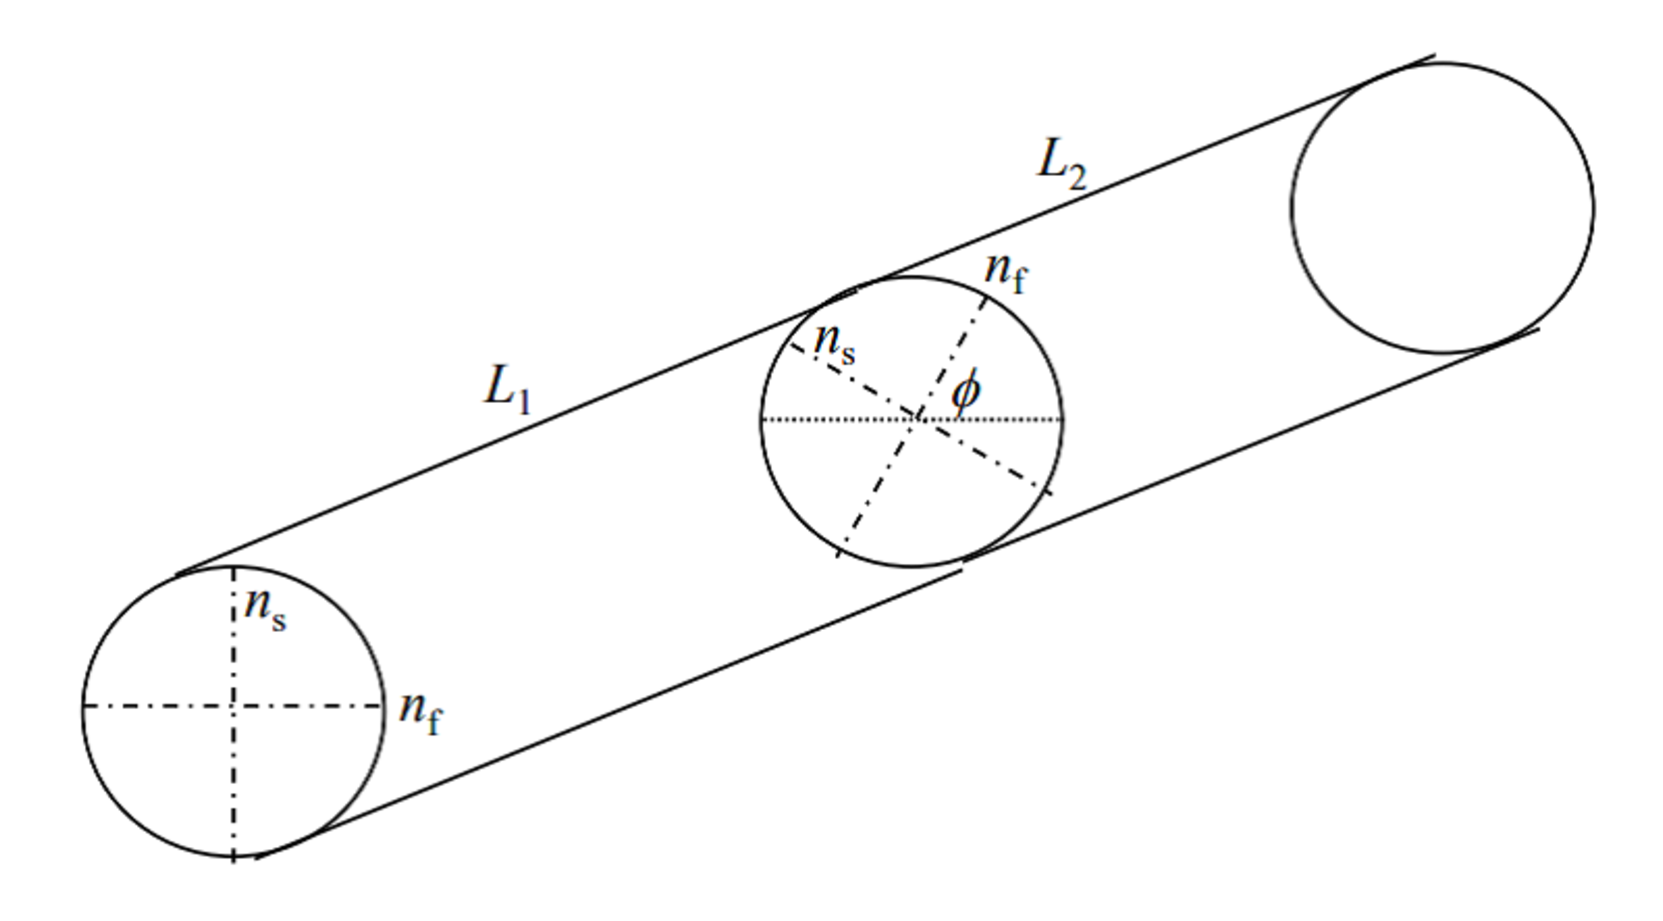
\includegraphics[width=100mm]{./figures/fig.eps}
    \end{center}
\end{figure}

\subsection*{解答}
\begin{enumerate}
    \renewcommand{\labelenumi}{(\alph{enumi})}
    \item
    1本目ファイバにおける偏波状態を$\bm{E_1}$とすると
    \begin{eqnarray*}
        \bm{E_1}(z=0)&=&(E_{1x}(0), E_{1y}(0))\\
        &=&(A, Ae^{-\frac{\pi}{2}i})e^{-i\omega t}
    \end{eqnarray*}
    ただし,ファイバの伝搬方向を$z$とする
    屈折率は$\{n_f, n_s\}$なので,1本目のファイバ伝送中の偏波状態は
    \begin{eqnarray*}
        \bm{E_1}(z)=(Ae^{in_fk_0z}, Ae^{-\frac{\pi}{2}i}e^{in_sk_0z})e^{i\omega t}
    \end{eqnarray*}
    よって,$L_1$伝搬後の偏波状態は
    \begin{eqnarray*}
        \bm{E_1}(L_1)=(Ae^{in_fk_0L_1}, Ae^{-\frac{\pi}{2}i}e^{in_sk_0L_1})e^{i\omega t}
    \end{eqnarray*}
    \item
    2本目のファイバは,主軸方向が$\phi$傾いているので\\
    接続境界においては
    \begin{eqnarray*}
        \left(\begin{array}{cc}E_{2x}(L_1)\\E_{2y}(L_1)\end{array}\right)=\left(\begin{array}{cc}\cos{\phi}&-\sin{\phi}\\\sin{\phi}&\cos{\phi}\end{array}\right)\left(\begin{array}{cc}E_{1x}(L_1)\\E_{1y}(L_1)\end{array}\right)
    \end{eqnarray*}
    \begin{eqnarray*}
        \bm{E_2}(L_1)&=&(E_{1x}(L_1)\cos{\phi}-E_{1y}(L_1)\sin{\phi}, E_{1x}(L_1)\sin{\phi}+E_{1y}(L_1)\cos{\phi})\\
        &=&(Ae^{in_fk_0L_1}\cos{\phi}-Ae^{-\frac{\pi}{2}i}e^{in_sk_0L_1}\sin{\phi}, Ae^{in_fk_0L_1}\sin{\phi}+Ae^{-\frac{\pi}{2}i}e^{in_sk_0L_1}\cos{\phi})e^{-i\omega t}        
    \end{eqnarray*}
    \item
    \begin{eqnarray*}
        \bm{E_2}(L_1+L_2)=(E_{2x}(L_1)e^{in_fk_0L_2}, E_{2y}(L_1)e^{in_sk_0L_2})
    \end{eqnarray*}
    \item
    $-\phi$だけ回転させると
    \begin{eqnarray*}
        \left(\begin{array}{cc}\cos{\phi}&\sin{\phi}\\-\sin{\phi}&\cos{\phi}\end{array}\right)\left(\begin{array}{cc}E_{2x}(L_1+L_2)\\E_{2y}(L_1+L_2)\end{array}\right)&=&\left(\begin{array}{cc}E_{2x}(L_1+L_2)\cos{\phi}+E_{2y}(L_1+L_2)\sin{\phi}\\-E_{2x}(L_1+L_2)\sin{\phi}+E_{2y}(L_1+L_2)\cos{\phi}\end{array}\right)\\
        &=&\left(\begin{array}{cc}E_{2x}(L_1)e^{in_fk_0L_2}\cos{\phi}+E_{2y}(L_1)e^{in_sk_0L_2}\sin{\phi}\\-E_{2x}(L_1)e^{in_fk_0L_2}\sin{\phi}+E_{2y}(L_1)e^{in_sk_0L_2}\cos{\phi}\end{array}\right)\\
        &=&\left(\begin{array}{cc}(Ae^{in_fk_0L_1}\cos{\phi}-Ae^{-\frac{\pi}{2}i}e^{in_sk_0L_1}\sin{\phi})e^{in_fk_0L_2\cos{\phi}}\\-(Ae^{in_fk_0L_1}\cos{\phi}-Ae^{-\frac{\pi}{2}i}e^{in_sk_0L_1}\sin{\phi})e^{in_fk_0L_2\sin{\phi}}\end{array}\right)e^{-i\omega t}\\
        &+&\left(\begin{array}{cc}(Ae^{in_fk_0L_1}\sin{\phi}-Ae^{-\frac{\pi}{2}i}e^{in_sk_0L_1}\cos{\phi})e^{in_sk_0L_2}\sin{\phi}\\(Ae^{in_fk_0L_1}\sin{\phi}-Ae^{-\frac{\pi}{2}i}e^{in_sk_0L_1}\cos{\phi})e^{in_sk_0L_2}\cos{\phi}\end{array}\right)e^{-i\omega t}
    \end{eqnarray*}
    % 下記の式を答えとして採用したいが,場所が無いので妥協
    % \begin{eqnarray*}
    %     =\left(\begin{array}{cc}\{(Ae^{in_fk_0L_1}\cos{\phi}-Ae^{-\frac{\pi}{2}i}e^{in_sk_0L_1}\sin{\phi})e^{in_fk_0L_2\cos{\phi}}\}+\{(Ae^{in_fk_0L_1}\sin{\phi}-Ae^{-\frac{\pi}{2}i}e^{in_sk_0L_1}\cos{\phi})e^{in_sk_0L_2}\sin{\phi}\}\\\{-(Ae^{in_fk_0L_1}\cos{\phi}-Ae^{-\frac{\pi}{2}i}e^{in_sk_0L_1}\sin{\phi})e^{in_fk_0L_2\sin{\phi}}\}+\{(Ae^{in_fk_0L_1}\sin{\phi}-Ae^{-\frac{\pi}{2}i}e^{in_sk_0L_1}\cos{\phi})e^{in_sk_0L_2}\cos{\phi}\}\end{array}\right)e^{-i\omega t}
    % \end{eqnarray*}
\end{enumerate}